% vim: ft=tex

\begin{figure*}[t]
  \centering
  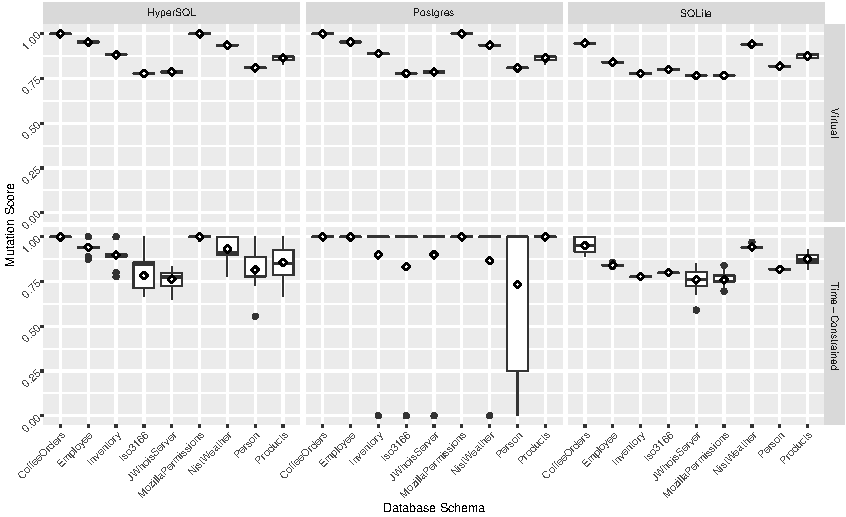
\includegraphics[scale=1.0]{graphics/graphic_bwplot_schema_mutationscore_vm_tcm.pdf}
  \caption{Box plot of the mutation score for the virtual and time-constrained mutation analysis techniques.}

  % Details about the box plot from the R documentation:

  % The lower and upper "hinges" correspond to the first and third quartiles (the 25th and 75th percentiles). This differs
  % slightly from the method used by the boxplot function, and may be apparent with small samples. See boxplot.stats for for
  % more information on how hinge positions are calculated for boxplot.

  % The upper whisker extends from the hinge to the highest value that is within 1.5 * IQR of the hinge, where IQR is the
  % inter-quartile range, or distance between the first and third quartiles. The lower whisker extends from the hinge to
  % the lowest value within 1.5 * IQR of the hinge. Data beyond the end of the whiskers are outliers and plotted as points
  % (as specified by Tukey).

  {\small \justifying{ \noindent In this plot the box itself represents the interquartile range (IQR), or the measure of
      statistical dispersion that is the difference between the first and third quartiles. Furthermore, the upper
      whisker extends from the top of the box to the highest value that is within 1.5 times the IQR and the lower
      whisker goes from the bottom of the box to the lowest value within 1.5 times the IQR. Finally, the thick
      horizontal line represents the median value, the filled circles denote outliers, and the open diamond is the mean
      value.}\par}

\end{figure*}


